\documentclass{article}
\usepackage{nips_2016}
% to compile a camera-ready version, add the [final] option, e.g.:
% \usepackage[final]{nips_2016}
\usepackage[utf8]{inputenc} % allow utf-8 input
\usepackage[T1]{fontenc}    % use 8-bit T1 fonts
\usepackage{hyperref}       % hyperlinks
\usepackage{url}            % simple URL typesetting
\usepackage{booktabs}       % professional-quality tables
\usepackage{amsfonts}       % blackboard math symbols
\usepackage{nicefrac}       % compact symbols for 1/2, etc.
\usepackage{microtype}      % microtypography
\usepackage{graphicx}


\newcommand{\tell}{\ensuremath{\tilde{\ell}}}

\newcommand{\w}{\mathbf{w}}
\newcommand{\G}{\mathbf{G}}
\newcommand{\x}{\mathbf{x}}
\newcommand{\g}{\mathbf{g}}
\newcommand{\R}{\mathbb{R}}
\newcommand{\tr}{{\!\top}}
\newcommand{\E}{\ensuremath{\mathbb{E}}}
\newcommand{\Exy}{\ensuremath{\mathbb{E}_{\x,y}}}
\newcommand{\BigBracks}[1]{\Bigl[#1\Bigr]}



\title{Learning to gentoype with SGD and linear models}

\author{
Nicol\'as Della Penna
\And
Erik Garrison \\
} %equal contributors


\begin{document}
% \nipsfinalcopy is no longer used

\maketitle

\begin{abstract}

  We present a process to transform the sequencing information used for genotyping new individuals into a feature representation that is suitable for experimentation in existing machine learning frameworks.
  The system is simple, has a fixed memory footprint, and can process millons of candidates per minute on a commodity compute cluster.
  We use an ablation study to explore the components of our feature representation that are important for good genotyping results.
  We demonstrate state of the art performance via participation in the first public competition focused on the genotyping task.
  
\end{abstract}

\section{Introduction}


%motivation

% TODO:why you care about genotyping,1 line.
Genome sequencing has rapidly become a core observational process in biology and medicine.
Sequencing and assembling a genome \emph{de novo} is dramatically more expensive than \emph{re}sequencing, in which the fragments of a newly-sequenced genome are aligned against an existing assembled reference genome).
As the error rates of sequencing methods are typically much higher than the rate of actual genetic variation, it is necessary to classify the candidate variations which are implied by the alignments on the basis of their veracity.
Organisms (such as humans) frequently have two or more nearly-identical copies of each genetic locus, and as a result we reason about their genome in as a series of genotypes, which are multisets of alleles $G = \{ a_1, \ldots, a_N \}$.\footnote{The same allele can occur more than once in diploids and polyploids.} 
% TODO: what learning task is genotyping ;   classification number of possible allelic states,

Let $N$ be the number of genome copies at a genomic locus, $A$ be the set of alleleic states where an alleles is a sequence of DNA, and $E$ be the set of degenerate or unknown states.
We obtain sequencing information $S$ relevant to our task by aligning small fragments of DNA to a reference genome \cite{li2013bwamem} or by building an assembly graph that compresses the input sequencing data before contextualizing it relative to the reference \cite{myers2005, simpson2010, li2015fermikit, iqbal2012}.
\emph{Genotyping} can be seen as an $N \times ( |A| + |E| )$-way classification task in which we use a model $f$ to obtain a mapping $f(S) \to G$.

%We can genotype a sample 

Standard approaches to developing $f$ use Bayesian filters derived from idealized \emph{a-priori} models of the genome  \cite{samtools, gatk2011, garrison2012haplotype, rimmer2014integrating, li2011stats}.
%This approach is sensible where we have little prior information to inform $f$, but ..
It is no longer the case that the best prior available for genome resequencing is one that we derive from first principles. 
Large scale genomic surveys have sequenced hundreds of thousands of humans, and where possible have deposited results into the public domain \cite{1000Gphase1, 1000g2015, exac2015, cavalli2005human, uk10k2015uk10k}.
The NIST Genome in a Bottle consortium \cite{zook2014integrating} has developed a reference standard for genome resequencing based around NA12878 (a cell line derived from a HapMap participant \cite{gibbs2003international}), which provides an accurate set of labeled data for the evaluation of genomic analyses.
Here, we develop a method to transform $S$ into a suitable feature space representation for efficient learning of $f$ and demonstrate the utility of our method by application to a public genomics challenge.

%To utilize this rapidly-deepening catalog of variation in a new individuals, we built a supervised learning task to genotype by example.

%President Obama’s Precision Medicine Initiative envisions a day when an individual's medical care will be tailored in part based on their unique characteristics and genetic make-up.
%The goal of the FDA's first precisionFDA challenge is to engage the genomics community in advancing the quality standards in order to achieve more consistent results in the context of genetic tests (related to whole human genome sequencing), advancing the goal of better personalized care.
%PrecisionFDA invites all innovators to take the challenge and assess their software on the supplied reference human datasets. Participation is voluntary, but instrumental in helping the community prepare for the coming genomic data revolution.

The PrecisionFDA challenge is a publicly-funded initiative to improve the quality and consistency of genetic tests through the engagement of the genomics community in a series of open challanges.
Its objective is to bring the same kind of rigorous public testing that has been used by the machine learning community to the medical genomics community.
We have applied our approach to the initial phase of the challenge (the ``Consistency'' challenge) and achieve the highest precision of any method which explicitly did not use the truth set in any phase of the submission process.\footnote{There was an entry that achieves 100 \% precision and recall by simply repeating the evlaution set, which was sadly distributed at the beginning of the challenge. Other submissions provide no more than vague reference to a ``ML'' approach used to filter, and do not exclude the use of the truth set for final decision boundary selection.}

%Our models base approach achieving the highest precision in the initial challenge (The precision challenge) of an entry that explciitly does not use the evaluation set in its training or paramter tunning 

%TODO https://precision.fda.gov/comparisons/1030 is problematic since they claim not to be using the test set (for training, i cosen my words crefully nd i assume so did they) 


%We require a corpus of examples of sequencing data from genomic loci where we have a strong estimate of the actual genome state. %TODO: edit flow with upper part
% this is available in NIST genome in a bottle
% background of problem
% history: 1000G, data formats, NIST
% current approaches 
% reference guided: bwa / aligners -> samtools, freebayes, platypus, GATK % assembly based: cortex, sga, fermikit
% similar techniques: GATK's VQSR (variant quality score recalibration) and SNPSVM (mention), but not a challenge particpant)
% VSQR provide rough idea of what is different http://gatkforums.broadinstitute.org/gatk/discussion/39/variant-quality-score-recalibration-vqsr
%The performance is comparable to that achieved by GATK with the recomended methodology; it offers several adavantges; libre, much smaller human effort, tunable to new sequencing tenchnologies (TODO: so is GATK's VQSR ...) 

The literature on genotyping is vast, and a full review of it is outside the scope of this paper.
Within the NIPS comunity \cite{teh2011modelling}, develop Bayesian nonparametric models for sequential data, the fragmentation-coagulation processes (FCPs), and a discrete time variant that mantains perofrmance while being more scalable. \cite{elliott2012scalable}
%http://papers.nips.cc/paper/4782-scalable-imputation-of-genetic-data-with-a-discrete-fragmentation-coagulation-process
In contrast, we take a discriminative instead of generative approach, and show that existing techniques as developed for large scale classification tasks can achieve state of the art performance when used with apropiately constructed features. 
As far as the methods have been described, none of the submissions to the FDA challenge so far appear to explicitly use these methods, nor come from groups that do so.

The discriminative approach has been used before in the intersection of machine learning and genomics, notably the Pascal learning challenge included a classficication task based on dna split point detection.
In contrast to that challenge that used a small set of 200 features, we explore models with up to hundreds of thousands of non-zero features per sample.
Further, the methods presented here are evauated not only in terms of performance metrics on the derived classification task, but rather as whole systems in open competition with custom designed software for the task that embodies dozens of human years of labor.

%Teh et al. (2011); Elliott & Teh (2012) showed that the Dirichlet diffusion tree (Neal, 2003b) is the fragementation-coagulation dual (Pitman, 2006; Bertoin, 2006) of the Kingman coalescent (Kingman, 1982; Teh et al., 2007). The stochastic process introduced therein can be viewed as combining the dual processes in order to model a time-evolving partition of objects. One could investigate if such a dual process exists for the beta diffusion tree or some variant thereof, from which a model for time evolving feature allocations could be obtained.

%TODO: how related is this? \cite{kirkpatrick2012bayesian} % http://papers.nips.cc/paper/4602-bayesian-pedigree-analysis-using-measure-factorization
%more broadly the " gene expression microarrays, " task % https://scholar.google.cz/scholar?q=gene&btnG=&hl=en&as_sdt=2005&sciodt=0%2C5&cites=15503184557873643836&scipsc=1


%Application papers should describe your work on a "real" as opposed to "hypothetical" application; specifically, it should describe work that has direct relevance to, and addresses the full complexity of, solving a non-trivial problem. Authors are also encouraged to convey insight about the problem, algorithms, and/or application

% elucidate (through an ablative analysis/lesion analysis, which removes one component of an algorithm at a time) which were the key components of the system needed to get the application to work. 
%The features provided by the two underlying aligners, combined with features that characterize the alignmnt itself, can be used to make a a good genotyper.



%A NIPS application paper should be comparable in quality to paper in the corresponding application domain conference: for example, a text paper should be acceptable to SIGIR, EMNLP, or other appropriate conference Application papers should not only present concrete application results, but also contain at least one of the below elements:

%Applications that couldn't previously be done, at all, or on this scale
%TODO can we argue somethign of what we are doing could be done before? at least not with libre software? or possibly theres some way to argue this.


%Techniques shown to be uniquely fitted to specific popular applications, leading to improved performance or more accurate solutions
%our strong point

%Insights that, from the perspective of machine learning, distinct applications X and Y, whose respective users have never talked to each other, are the same.
%cant see anythign like this, but leaving it for inspiration




%dna/gene literature in NIPS



\section{From sequencing machine to feature representation}

We transform the short reads derived from an Illumina sequencing platform into a feature space representation suitable for use by generic machine learning techniques in two phases.
In the first phase, we use standard techniques for the processing of sequencing data to project sequencing information from a new sample onto the reference genome.
We then use alignment and assembly based genotyping programs to derive a list of putatively variable sites and non-reference alleles at these sites.
In the second phase, we convert the alignments, assembly, and candidate alleles derived from the first phase into a text-based feature representation compatible with the Vowpal Wabbit.
The two steps are decoupled, allowing us to change the inputs to the feature space transformation by utilizing other tools or sources for candidate alleles.
The process can thus be understood as a generic ensemble genetic variant detection and genotyping platform, however in this application we explore the use of only a small set of sources for this information.

\subsection{Alignment, assembly, and variant calling}

We align reads to a reference genome using {\tt bwa mem} \cite{li2013bwamem} and mark PCR duplicates with {\tt bamsormadup} \cite{tischler2014biobambam}.
We then use {\tt freebayes} \cite{garrison2012haplotype} to derive candidate alleles and genotypes for all sites where we observe more than 2 reads supporting a non-reference allele that comprising at least 5\% of the sequencing data at the locus.
In parallel, we generate an assembly of the raw sequencing reads using {\tt fermikit} \cite{li2015fermikit}.
We then map uniquely contiguous stretches of non-branching sequence in the overlap graph (unitigs) back to the reference genome, and use these alignments to identify candidate alleles with a genotyping approach implemented in the {\tt fermikit} toolchain.
In addition to a set of per-site annotations about the read evidence that they are presented, both {\tt fermikit} and {\tt freebayes} provide a quality estimate in their outputs which is approximately the posterior probability of variation at the locus under their Bayesian models.
We threshold the results at an extremely low posterior probability ($\approx 10^{-8}$) so as to certain false positives that only increase the computational burden of learning.\footnote{When comparing to the NIST Genome in a Bottle truth set we observed no true positives in this region of the data.}
Finally, use tools in {\tt vcflib} to merge the results into a single set of candidates \cite{vcflibgit}, retaining software level annotations provided by both systems.

This toolchain is the simplest that we are aware of that combines the two main forms of genotyping in common use.
{\tt freebayes} implements a haplotype-based genetic variant detection process that examines only reads locally mapped to a particular locus, and is limited to detecting genetic variants that are approximately the same size as a single read.
This provides in high sensitivity to small variation.
In contrast, {\tt fermikit} compresses sequencing data into a string graph \cite{myers2005}, then projects the unique portions of this graph onto the reference to find potential sequence variants.
The compression reduces the sensitivity of the method to shorter sequence variants, which resemble sequencing errors, but through assembly of long stretches of DNA it is able to detect very large sequence variants, such as insertions and deletions of 10s of thousands of base pairs.
Both methods and the integration process we use are fully implemented using free software with permissive licensing, unlike similar solutions such as the {\tt GATK} \cite{gatk2011}, which will enable their free use by other researchers.

\subsection{A generic feature representation for genotyping}

Existing learning techniques to approximate $f(S) \to G$ only use aggregate statistics describing $S$ at the level of a single genomic site.
For instance, SNPSVM applies a support vector machine to site level annotations such as read depth and mean sequencing base quality \cite{o2013support}.
The {\tt GATK} Variant Quality Score Recalibrator (GATK-VQSR) uses a very similar feature space, but develops a site level quality ``recalibration'' by applying a guassian mixture model built from distributions learned on many genomes to estimate outlier variants given a known set of true positives.
The full read information $S$ is apparently considered to expensive to directly use as an input to learning.

However, we observed that bioinformaticians would often evaluate the quality of genotyping results using visual representations of read alignments such as those implemneted in {\tt IGV} or {\tt samtools tview} \cite{robinson2011integrative, samtools}.
The human-driven assertion that the site was ``good'' or ``bad'' based on the appearance of the alignments suggested that we could learn to genotype directly from the alignments.
Following this inspiration, we designed a feature representation that retains all relevant features of $S$.
We implement this transformation in a software tool that consumes alignments (in BAM format), candidate variants (in VCF format), a window size parameter $w$, and a maximum depth $d$ to produce a feature representation for each candidate containing a description of: the reference genome; candidate alleles from the VCF file; alignments and their matches to the candidate alleles and reference; software provided annotations from the VCF file; and a novel compression of the sequencing data against a sequence graph implied by the variant record.

Figure \ref{fig:indel} provides a visual explanation of the relevant parts of our feature space transformation, which we describe here in detail.


\begin{figure}[t]
\centering
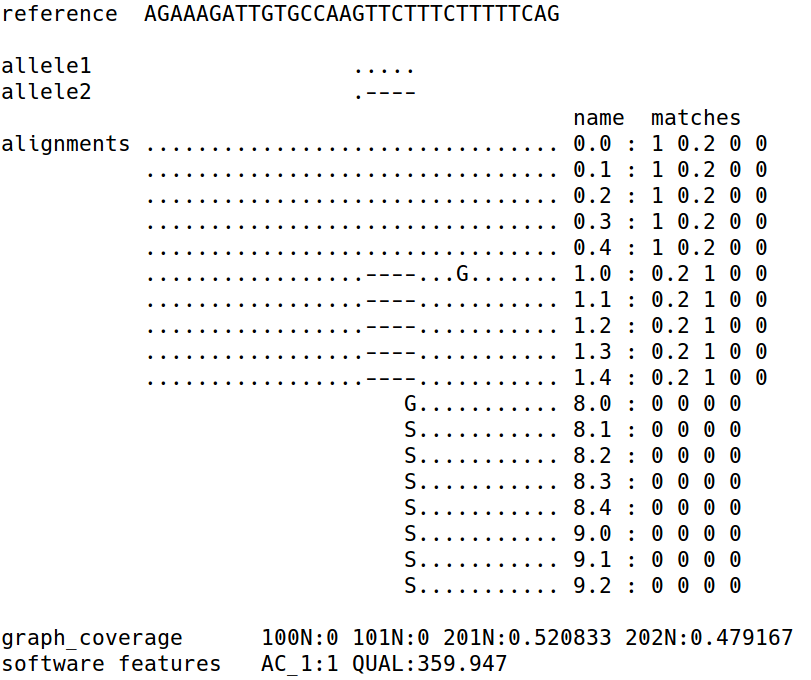
\includegraphics[width=1.0\textwidth]{indel}
\caption{\label{fig:indel}
  A human-readable fragment of the feature space transformation at a candidate indel site.
  The reference sequence is represented at top, the two candidate alleles from the VCF (allel1 is equal to the reference and the other features a relative deletion).
  The alignment name which is derived from the match-invariant sort and the match features are shown to the right of the matrix.
  Below the alignment matrix is a representation of the variation graph and software-derived features.
}
\end{figure}

\subsubsection{The alignment matrix}

% hra

At each locus we generate a mutually gapped reference-based multiple sequence alignment (MSA) of the alignments, reference, and candidate alleles from the VCF file using the same algorithm as that implemented in {\tt samtools tview}.
We build the matrix using the alphabet $\{ {\tt A, T, G, C, N, U, M, R, S} \}$.
$\{ {\tt A, T, G, C} \}$ represent the standard DNA bases where the alignment suggests a candidate single base change (SNP), ${\tt N}$ is a degenerate character that could represent any of the standard bases, ${\tt U}$ is a gap character used to pad the alignment matrix where sequences have relative insertions or deletions (indels), ${\tt M }$ indicates missing data, ${\tt R}$ represents a reference-matching base in an alignment, and ${\tt S}$ indicates a ``soft clip'' or insertion at the beginning or end of an alignment.
This MSA is represented in matrix form, with its width equal to the window size and depth bounded by the number of alignments or an optional parameter that caps the number of alignments passed through the feature transformation.

To build the mutually gapped MSA, we first record all unique edits between the reference genome and the alignments.
Then, we determine the edit with the longest insertion length relative to the reference at each position and gap the alignments and reference at that position by adding the gap character ${\tt U}$ to them where their sequence length at the position is less than the maximum insertion length.
We use the same gap character to indicate relative deletions between the alignments and the reference.
We pad the alignments and candidate alleles with ${\tt M}$ where they do not fully overlap the window.

The mutual gapping step may change the width and centering of the matrix, so we must re-center and bound it.
We center the matrix such that the first base pair in the VCF record which we are working from is $w/2$ characters from the left hand edge of the window.
Finally, we re-bound the matrix so that it contains $w$ columns.
In effect, the variation is always represented in the right side of the matrix.

We build the matrix in the same way for small variants such as SNPs as we do for longer variants such as indels.
Although much of a longer indel will not be represented, we can use the first $w/2$ base pairs of it when genotyping.
For a typical window size $w = 16$, this would provide us 8 base pairs of information from each alignment.
As most indels are short, this will only harm resolution for long indels.

\subsubsection{Candidate-relative alignment sort}

% m

We sort the alignment matrix in a way that provides an approximate invariance relative to matches between the alignments and the candidate alleles.
For each alignment, we determine its pairwise identity with all candidate alleles.
For each candidate allele, we then sort the alignments in descending order by their match rate to the candidate alleles.
We then project the gapped alignments from the MSA into one matrix per allele where each matrix contains the top $d$ alignments sorted by match with that allele.
Alignments that do not match any candidate allele are sorted into another matrix, as are alignments which contain soft clips.
We sort soft clips separately because they are used by several methods to detect larger variants \cite{kronenberg2015wham}, which we hypothesized would help when genotyping variants detected by assembly with {\tt fermikit}.
All alignment-relative features are provided in this sort order.
We provide the match rates between each alignment and each candidate allele in the same order as the the alignments are sorted in the candidate-relative invariant sort.

\subsubsection{Software-provided annotations}

% s

We map software provided annotations provided in the VCF directly into a feature space in our representation.
Thes features include the estimated posterior probability of variation at the locus, the read depth, the sum of base qualities in the alignments, and other aggregate point statistics that the method developer has provided.

\subsubsection{Variation graph compression}

% k

The mutually gapped alignment matrix is susceptible to noise in the alignments.
Indel errors influence the representation of all other alignments, which makes the representation unstable.
Additionally, as we use the reference-based alignments to build up the alignment matrix representation, the representation is susceptible to errors in alignment.
As the alignments are derived between the reference and each read, they do not benefit from the information about candidate variation.
We resolve these issues by generating a ``variation graph'' that exactly represents the VCF record and aligning the reads against it in order to generate a compressed and fully normalized representation of the aggregate relationship between the alignments and candidate alleles.

We define a variation graph to be a graph with embedded paths $G = ( N, E, P )$ comprised of
a set of nodes $N = n_1 \ldots n_M$,
a set of directed edges $E = e_1 \ldots e_L$,
and a set of paths $P = p_1 \ldots p_Q$ which describe transformations from the graph space into a set of sequences.
Each node $n_i$ represents a sequence $seq(n_i)$ which is built from an arbitrary alphabet ${ \cal A } = \{ {\tt A, T, G, C, N} \}$.
Edges represent linkages between nodes that are allowed to be followed in representing longer sequences as paths through the graph.

We are interested in alignments to this graph, which we describe as alignments to a walk (or path) through the graph.
Explicitly, a path is a series of ``mapping'' operations, each describing the segment of the path derived from a single node, $p = m_1, \ldots, m_{|p|}$.
Each mapping $m$ can be written as $( (n, o), e_i \ldots e_{|m|} )$, where $n$ is the node, $o$ is the zero-offset start position on the node ($0 \le o < |n|$), and each $e_i$ is an ``edit'' which copies or replaces a segment of the node sequence.
This model is a straightforward generalization of the pairwise alignments generated by reference-based aligners to operate on a graph.

For each site we construct a graph $G$ such that the reference and alleles are represented as paths through the graph.
We construct the graph such that the alleles in the VCF record are whole nodes and the reference flanks around the locus are the single head and tail nodes of the graph.
We then collect reads that map within a larger window $g : g > w$ around the center of our window and realign them to $G$ using an efficient implementation of partial order alignment (POA) \cite{lee2002POA}.\footnote{In practice we use $g = 100$.}
As we aim to obtain a relativistic description of the strength of match between the alignments and the specific alleles at the locus, we ignore any edits in the alignments.
We then count the number of alignments mapping to each allele node, and normalize these counts by the total number of alignments mapping to any allele node.
This results in a weight $k$ for each allele node such that $k_i \in [0, 1] \forall n_i \in N$ and $\sum_{i = 0}^{|A|} k_i = 1$, which we provide in the feature representation.

\begin{figure}[t]
\centering
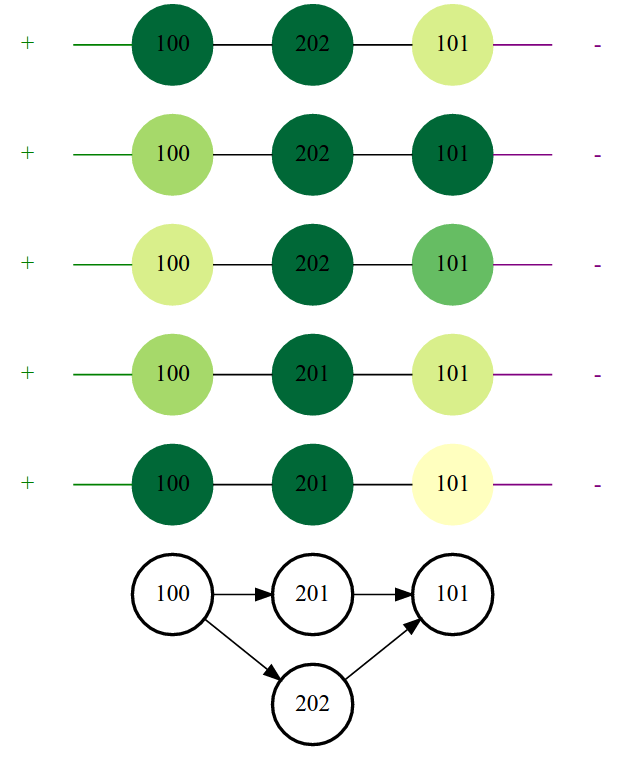
\includegraphics[width=0.5\textwidth]{graphaln}
\caption{\label{fig:graphaln}
  A representation of the alignment of 5 reads to the variation graph in figure \ref{fig:indel}.
  Nodes 100 and 101 are the flanking reference nodes, while nodes 201 and 202 are the candidate allele nodes.
  Sequences are not shown.
  The color of the nodes indicates the quality of the match in the alignnment for that node in the graph, with green representing good matches and lighter colors representing poorer matches.
  In this case 3 reads map to node 202 and 2 reads map to node 201, so we would derive a representation of this data as 201N:0.6 202N:0.4 in our feature space.
}
\end{figure}

\subsection{Application to PrecisionFDA Consistency Challenge}

% notes from precisionFDA
For the PrecisionFDA Consistency Challenge, participants were tasked with producing high-quality and reproducible genotyping results for a new sequencing data set derived from the canonical NA12878 reference cell line.
In effect, the objective was to test the ability of methods to generalize across different sequencing runs.\footnote{An ongoing challenge, the ``Truth'' challenge, seeks to measure generalization across individuals. It will close on May 26th, 2016, so we are unable to provide results at the time of this submission.}

To answer the challenge, we trained the models using three previous Garvan Institute sequencing runs on NA12878.\footnote{We used data available at https://www.garvan.org.au/research/kinghorn-centre-for-clinical-genomics/clinical-genomics/sequencing-services/sample-data for Robot\_1, Robot\_3, and Robot\_4.}
We labeled the candidate loci with their genotype status in the NIST Genome in a Bottle v2.19 truth set for NA12878 and use the learning procedure described in \ref{sec:learning} to train a model using only the previously-available data from the Garvan Institute.
We generated the feature transformation in the same manner for the challenge test data (Vial\_1), and derived labels for the candidates using the model trained on the previously-available data.
Finally, we convert the results into the VCF format and uploaded them into the PrecisionFDA testing framework.
There we used a remote comparison tool hosted by the organizers to evaluate the results.
This provides three metrics: precision (the percent of correct genotypes in the total set), recall (the fraction of precise genotype and allele assignments out of the total possible in the truth set) and an F-measure that combines the two under the assumption of equal weight for false positives and false negatives.
In our submission we achieve a precision of 99.54\%, recall of 98.91\% and an F-measure of 99.22\%.
Furthermore, we achieve the highest precision of any group that explicitly did not use the truth set (Vial\_1) in selecting parameters or thresholds for the submission.

\section{Learning}
\label{sec:learning}


The learning is carried out with feature hashing and stochastic gradient descent using adaptive normalized and invariant update scheme as implemented in Vowpal Wabbit \cite{mcmahan2010adaptive, duchi2011adaptive, agarwal2014reliable}

Each of the variables in the feature sets implemented above along with a quadratic terms for their values, and a set of cross interactions where, as well as 2-grams over the sequence like features  is included in a vector $x$.
The hashing trick is used to carry out the projection.
Stochastic gradient descent then optimizes a set of weights $w$ so as to:

\begin{equation}
  \min_{\w \in \R^d}~~\sum_{i=1}^n\ell(\w^\tr\x_i;\,y_i)
  \label{eqn:objective}
\end{equation}

Note that this is without any explicit regularization penalty.
Capacity control is instead carried out by stopping the iterations of the gradient descent when the holdout error rate is not reduced over three iterations \citep{hardt2015train}.
For the very largest models (those that include quadratic features of the allele reads) the saturation of the hash space also potentially provides a for of capacity control.
The main reason behind this choice was to avoid hyper-parameter tuning given the computational cost of fitting the richer models (thousands of CPU core hours).

Error-correcting tournaments \citep{beygelzimer2009error} where used,  despite the small number of classes, this showed better performance in the holdout than the standard one against all reductions in our initial experiments.
Comparisons of our final models show that the performance with respect to the more standard one is withing 0.01\% of each other on binary loss.

%Feature hashing and stochastic gradient descent using adaptive normalized and invariant update scheme as implemented in Vowpal Wabbit \cite{mcmahan2010adaptive, duchi2011adaptive, agarwal2014reliable} 


\section{Results}

Table \ref{tab:ablate} presents a range of models to provide a sense of the importance of the different features used.
We report loss on large held out regions of the genome (100/827 regions are held out), as this is the best-available proxy for another individual until the projected release of the second NIST truth set in late May 2016.
Our objective with this holdout strategy is to develop intuition about generalization across different individuals.
All experiments were carried out using the synchronous cluster mode for VW using either 30 or 300 concurrent learners.

We expect the reference and candidate allele features to provide little generalization ability to new regions of the genome, which is held out by the results.
Software level annotations provide a compact and discriminant representation of $S$.
The alignments alone provide sufficient power to achieve 1.7\% error, which is similar to the error rates achieved by {\tt freebayes}, {\tt fermikit}, and other Bayesian variant callers.
The variation graph compression is vastly more compact than the alignment feature with an average of 2 vs 1000s of non-zero features per example, but achieves only slightly worse performance, perhaps because it cannot capture context specific errors which are evidenced by certain motifs in the alignments \cite{nakamura2011sequence}.

%The best performance is achieved by using 

\begin{table}[]
  \centering
  \caption{Baselines \& Ablations }
  \label{tab:ablate}
  \begin{tabular}{|l|l|l|l|l|}
    \hline
    name & 0/1 loss & feature spaces & interactions & options \\ \hline
    Software-provided annotations & 0.012204 & s & ss & \\
    Reference  & 0.407825 & r & rr &\\
    Alignments & 0.016569 & a & & \\
    Allele & 0.416780 & h & hh & \\
    Variation graph compression & 0.035268 & k & kk & \\
    Candidate-relative alignment match & 0.024088 & m & mm & \\
    Match and software & 0.009975 & ms & mm  ss  ms & \\
    Variation graph and Cand. Align. & 0.021169 & km & kk  mm  km & \\
    ... and software & 0.009639 & kms & kk  km  mm  ms  ss & \\
    ... and soft. and reads & 0.008795 & kmsa & kk  km  mm  ms  ss & \\
    with alleles & 0.009060 & kmshr & kk  km  mm  ms  ss  hr & \\
    .... 2-grams  & 0.009205 & kmshr & kk  km  mm  ms  ss  hr & ngram 2 \\
    ... 3-grams & 0.009368 & kmshr & kk  km  mm  ms  ss  hr & ngram 3 \\
    ... alle reads and 2 grams  & 0.008799 & kmshra & kk  km  mm  ms  ss  hr & ngram 2 \\
    Growing polynomials & 0.012261 & kmshr & & stage-poly \\
    \hline
  \end{tabular}
\end{table}

% can't do ... maybe we report it -- effect of using "clever" featuranmes for aln relative to just some natural ordering.



%that's enough to make a strong claim that you would generalize to a new sample with different variants in different places
%if you want to go so far
%obviously it has caveats but if you want to explore this that's the cleanest way

%that DNA is a molecule and when a person has a variatn in a new position it is indistinguishable from another variant we held out from the current individual

%the itner-individual comparison in the 1000G is fraught too
%because the samples were all genotyped in a massive joint assembly process
%so it's hard to claim they are independent

\section{Conclusion}

Using simple, shallow learners, and leveraging the work that has been applied to large scale classification tasks combined with handcrafted feature representations, we show state of the art performance in genotyping task.
We present the first method to solve this problem in a way that retains information about the source data through the feature trasnformation, development, and application of a model.
Our experiments show that this information alone is suitable for use in a simple learner.

%\section{Further Work}
%incoporating 1000G


%somehow bring in?
%Teh et al. (2011); Elliott & Teh (2012) showed that the Dirichlet diffusion tree (Neal, 2003b) is the fragementation-coagulation dual (Pitman, 2006; Bertoin, 2006) of the Kingman coalescent (Kingman, 1982; Teh et al., 2007). The stochastic process introduced therein can be viewed as combining the dual processes in order to model a time-evolving partition of objects. One could investigate if such a dual process exists for the beta diffusion tree or some variant thereof, from which a model for time evolving feature allocations could be obtained.


\small

\bibliographystyle{plain}
\bibliography{geno}

\end{document}


